\documentclass[__main__.tex]{subfiles}

\begin{document}

\section{Область с липшицевой границей. Примеры. Пространство L 2 . Обобщенные производные. Лемма о единственности обобщенной производной. Пространства Соболева $H^k$ (два эквивалентных определения). Простейшие свойства пространств Соболева. Теорема Грина. Неравенство Фридрихса. Неравенство Корна.}

\begin{definition}
	\textbf{Область с липшицевой границей.} Пусть $\Omega \in \mathbb{R}^{n}$ - ограниченная область , для которой существуют m декартовых систем координат $(X_{1}^{(r)},..,X_{n}^{(r)})$  r =1..m и $\alpha,\beta \in \mathbb{R}$, m функций $a_{v}(X_{1}^{(r)},..,X_{n-1}^{(r)})$ непрерывных в кубах $K_{r}={|X^{r}_{i}|<\alpha, i=1...n-1}$ и таких что:\\
	\textbf{1)} $\forall x\in \partial\Omega \exists r=1..m,$ что $x=(X_{1}^{(r)},..,X_{n-1}^{(r)},a_{v}(X_{1}^{(r)},..,X_{n-1}^{(r)}))$\\
	\textbf{2)} $\forall x=(X_{1}^{(r)},..,X_{n-1}^{(r)}), r=1..m ,$ для которых $x\in K_{r} и X^{r}_{n} \in (a_{v}(X_{1}^{(r)},..,X_{n-1}^{(r)}),(X_{1}^{(r)},..,X_{n-1}^{(r)})+\beta)$ или \\
	$X^{r}_{n} \in (a_{v}(X_{1}^{(r)},..,X_{n-1}^{(r)})- \beta,a_{v}(X_{1}^{(r)},..,X_{n-1}^{(r)}))\rightarrow x \in \Omega$ / $\partial\Omega$ либо $x \notin \vec{\Omega}=\Omega \vee \partial\Omega$\\
	\textbf{3)}	$\forall x,y \in K_{r},$ r=1..m\\
	$|a_{v}|(X_{1}^{(r)},..,X_{n-1}^{(r)})-a_{v}|(Y_{1}^{(r)},..,Y_{n-1}^{(r)})\leq$  \ L\ ||x-y||

\textbf{Примеры}
\begin{figure}[H]
	\centering
	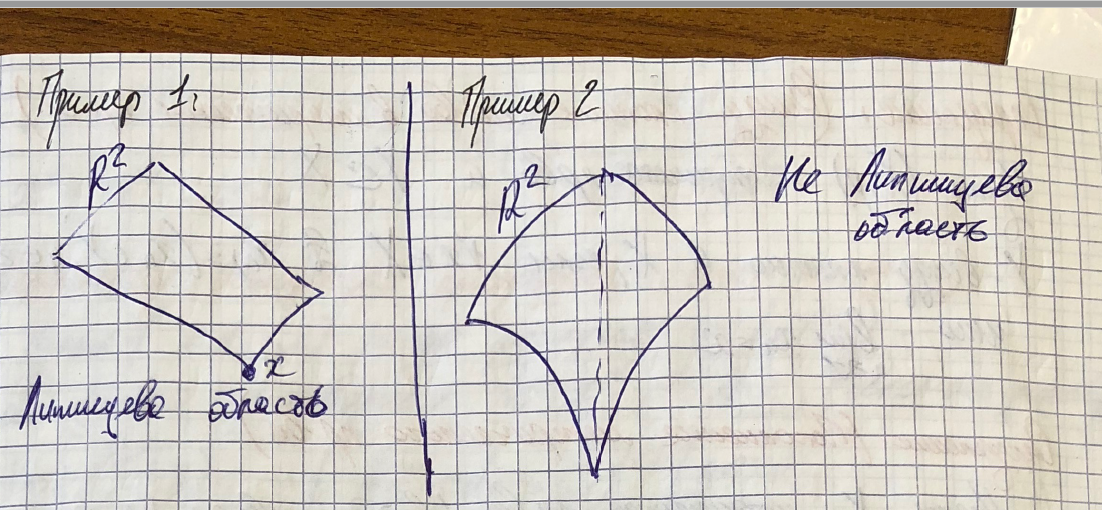
\includegraphics[width=0.7\linewidth]{screenshot001}
	\caption{}
	\label{fig:screenshot001}
\end{figure}

\end{definition}

\begin{definition}
\textbf{$L_{2}$}($\Omega)$. Множество функций x:$\Omega\rightarrow\mathbb{R}$, таких что $x^{r}$ - интегрируема по Лебегу со скалярным произведением $(x,y)=\int_{\Omega}x(\tau)y(\tau)d\tau$
\end{definition}

\begin{definition}
\textbf{Обобщенная производная (n-го порядка)}. Пусть $f\in L_{2}(\Omega)$, тогда функция $q \in L_{2}(\Omega)$ называется обобщенной производной f по $x^{\alpha},|\alpha|=n,$ , если $\forall v \in C_{0}^{\infty}(\Omega)$ - финитная бесконечно дифференцируемая\\
$\int_{\Omega}f\partial^{\alpha}v d\tau = (-1)^{|\alpha|}\int_{\Omega}qvd\tau$.\\
Тогда q обозначается: $q=\partial^{\alpha} f$ 
\end{definition}

\begin{definition}
\textbf{Пространством Соболева $H^k$}. Подмножество элементов $f\in L_{2}(|\Omega|),$ имеющих обобщенные производные $\partial^{\alpha}\ \forall \alpha: |\alpha|=k$ со скалярным произведением: \\
$(f,q)_{H^{k}(\Omega)}=\sum_{|\alpha|\leq k}(\partial^{\alpha}f,\partial^{\alpha}q)_{L_{2}(\Omega)}$\\
называется \textbf{пространством Соболева $H^k$}
\end{definition}

\begin{definition}
Пусть на $X=C_{0}^{\infty}(\Omega)$ введено скалярное произведение :\\
$$(f,q)=\sum_{|\alpha|\leq k}\int_{\Omega}\partial^{\alpha}f \partial^{\alpha}q d\tau,  \forall f,q\in X$$\\
Тогда пополнение пространства (X,$\rho$), $\rho(x,y)^{2}\leq(x-y,x-y)$ называется \textbf{пространством Соболева $H^k$}.  
\end{definition}

\textbf{Свойства пространств Соболева}\\
$T_{r_{\partial\Omega}}:H^{1}(\Omega)\rightarrow L_{2}(\Omega)$ - след. Причем  $T_{r_{\partial\Omega}}$ - ограничен и если $f\in C^{\infty}_{0}(\Omega),$ то 
$(T_{r_{\partial\Omega}}f)(s)=f(s),  \forall s\in \partial\Omega $\\
$f\in H^{1}(\Omega),  q-$обобщенная производная. $q=T_{r_{\partial\Omega}} f,$то $||q||_{L_{2}(\partial\Omega)}\leq M||f||_{H^{1}(\Omega)},$ M - const.

\begin{theorem}
	\textbf{Теорема Грина.} Пусть f,q (обобщенная производная) $\in H^{1}(\Omega),$тогда 
	$$\int_{\Omega}f\frac{\partial q}{\partial x_{i}}d\tau=-\int_{\Omega}q\frac{\partial f}{\partial x_{i}d}\tau+\int_{\partial\Omega}fq n_{i}d\tau	\ , i=1..n,$$ 
	$n_{i}$- компоненты вектора единичной нормали к $\partial\Omega$.
\end{theorem}
\begin{theorem}
\textbf{Неравенство Фридрихса}. $\Omega \in \mathbb{R}^{n}$- область. Пусть $f\in H^{1}(\Omega),\Omega$- область с липшицевой границей, Г$\in\partial\Omega$.\\
$\mu ($Г$)\neq 0$, тогда справедливо неравенство 
$$||f||^{2}_{H^{1}()\Omega}\leq C(\Omega,\textit{Г})(\sum_{i=1}^{n}\int_{\Omega}(\frac{\partial f}{\partial x_{i}})^{2}d\tau+\int_{\text{Г}}q^{2}(s)ds)$$, q(s) - обобщенная производная, C($\Omega,$Г)=const
\end{theorem}

\begin{theorem}
\textbf{Неравенство Корна} Пусть $\Omega$ - липшицева область, Г$\in\partial\Omega$ - часть границы этой области, такая что $\mu(\text{Г})\neq0$ -мера.\\
Тогда $\forall \vec{u}\in [H^{1}(\Omega)]^{3}:T_{r_{\text{Г}}}u_{i}=0$ справедливо неравенство \\
$$\sum_{i,j}^{3}\int_{\Omega}\epsilon_{i,j}^{2}(u)d\tau\geq C_{k}||\vec{u}||_{[H^{1}(\Omega)]^{3}}$$\\
$C_{k}=$const - коэффициент нормирования.
\end{theorem}


\end{document}
